
\begin{figure}[htp]
    \begin{minipage}[t]{0.47\textwidth}
    \centering
    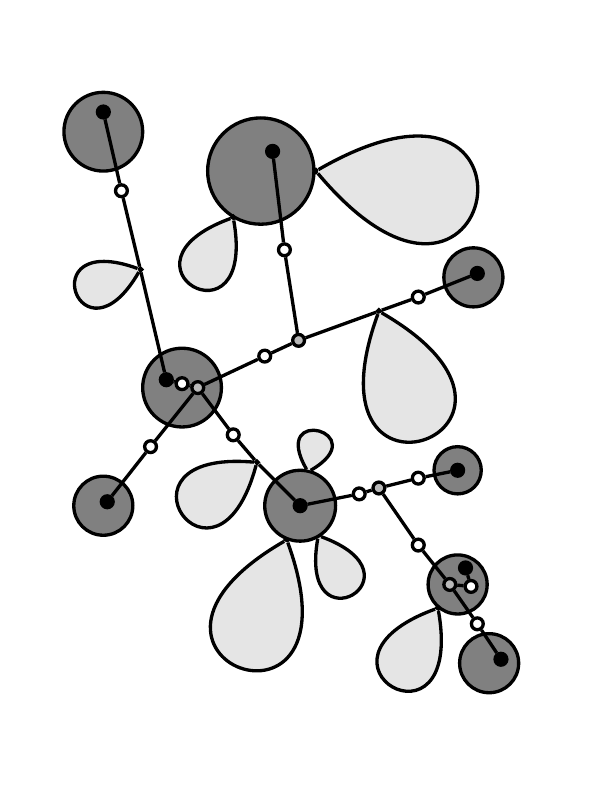
\begin{tikzpicture}[every node/.style={draw, very thick}, every path/.style={very thick}]
    
    \node[circle, draw, minimum size = 1cm, fill=gray] (1) at (-3,2.75) {};
    \node[circle, draw, minimum size=0.15cm, inner sep=0pt, fill=black] (2) at (-3,3) {};

    
    
    \node[circle, draw, minimum size = 1.35cm, fill=gray] (3) at (-1,2.25) {};
    \node[circle, draw, minimum size=0.15cm, inner sep=0pt, fill=black] (4) at (-0.85,2.5) {};
    \node[circle, draw, inner sep=0pt, fill=white] (36) at (-0.3,2.25) {};
    \node[circle, draw, inner sep=0pt, fill=white] (40) at (-1.35,1.66) {};
    

    
    \node[circle, draw, minimum size=0.15cm, inner sep=0pt, fill=white] (5) at (-2.77,2) {};
    
    \node[circle, draw, minimum size=0.15cm, inner sep=0pt, fill=white] (6) at (-0.7,1.25) {};
    
    \node[circle, draw, minimum size = 0.75cm, fill=gray] (7) at (1.7,0.9) {};
    \node[circle, draw, minimum size=0.15cm, inner sep=0pt, fill=black] (8) at (1.75,0.95) {};
    
    \node[circle, draw, inner sep=0pt, fill=white] (9) at (-2.53,1) {};
    
    \node[circle, draw, minimum size=0.15cm, inner sep=0pt, fill=white] (10) at (1,0.65) {};
    
    \node[circle, draw, inner sep=0pt, fill=white] (11) at (0.5,0.47) {};
    
    \node[circle, draw, minimum size=0.15cm, inner sep=0pt, fill=gray!55] (12) at (-0.52,0.1) {};
    
    \node[circle, draw, minimum size=0.15cm, inner sep=0pt, fill=white] (13) at (-0.95,-0.1) {};

    
    \node[circle, draw, minimum size = 1cm, fill=gray] (14) at (-2,-0.5) {};
    \node[circle, draw, minimum size=0.15cm, inner sep=0pt, fill=black] (15) at (-2.2,-0.4) {};
    \node[circle, draw, minimum size=0.15cm, inner sep=0pt, fill=white] (16) at (-2,-0.45) {};
    \node[circle, draw, minimum size=0.15cm, inner sep=0pt, fill=gray!55] (17) at (-1.8,-0.5) {};
    
    \node[circle, draw, minimum size=0.15cm, inner sep=0pt, fill=white] (18) at (-1.35,-1.1) {};

    \node[circle, draw, minimum size=0.15cm, inner sep=0pt, fill=white] (19) at (-2.4,-1.25) {};
    
    \node[circle, draw, inner sep=0pt, fill=white] (20) at (-1.05,-1.45) {};
    
    \node[circle, draw, minimum size = 0.6cm, fill=gray] (21) at (1.5,-1.55) {};
    \node[circle, draw, minimum size=0.15cm, inner sep=0pt, fill=black] (22) at (1.5,-1.55) {};
    
    \node[circle, draw, minimum size=0.15cm, inner sep=0pt, fill=white] (23) at (1,-1.65) {};
    
    \node[circle, draw, minimum size=0.15cm, inner sep=0pt, fill=gray!55] (24) at (0.5,-1.775) {};
    
    \node[circle, draw, minimum size=0.15cm, inner sep=0pt, fill=white] (25) at (0.25,-1.85) {};

    \node[circle, draw, minimum size = 0.75cm, fill=gray] (26) at (-3,-2) {};
    \node[circle, draw, minimum size=0.15cm, inner sep=0pt, fill=black] (27) at (-2.95,-1.95) {};
    \node[circle, draw, inner sep=0pt, fill=white] (41) at (-0.67,-2.433) {};
    \node[circle, draw, inner sep=0pt, fill=white] (42) at (-0.27,-2.38) {};
    \node[circle, draw, inner sep=0pt, fill=white] (43) at (-0.4,-1.57) {};
    
    \node[circle, draw, minimum size = 0.9cm, fill=gray] (28) at (-0.5,-2) {};
    \node[circle, draw, minimum size=0.15cm, inner sep=0pt, fill=black] (29) at (-0.5,-2) {};

    
    \node[circle, draw, minimum size=0.15cm, inner sep=0pt, fill=white] (30) at (1,-2.5) {};
    
    \node[circle, draw, minimum size = 0.75cm, fill=gray] (31) at (1.5,-3) {};
    \node[circle, draw, minimum size=0.15cm, inner sep=0pt, fill=gray!55] (32) at (1.4,-3) {};
    \node[circle, draw, inner sep=0pt, fill=white] (37) at (1.25,-3.3) {};
    \node[circle, draw, minimum size=0.15cm, inner sep=0pt, fill=black] (38) at (1.6,-2.79) {};
    \node[circle, draw, minimum size=0.15cm, inner sep=0pt, fill=white] (39) at (1.67,-3.025) {};
    
    \node[circle, draw, minimum size=0.15cm, inner sep=0pt, fill=white] (33) at (1.75,-3.5) {};
    
    \node[circle, draw, minimum size = 0.75cm, fill=gray] (34) at (1.9,-4) {};
    \node[circle, draw, minimum size=0.15cm, inner sep=0pt, fill=black] (35) at (2.05,-3.95) {};
    
    \draw[] (2) to (5);
    \draw[] (4) to (6);
    \draw[] (5) to (9);
    \draw[] (6) to (12);
    \draw[] (8) to (10);
    \draw[] (9) to (15);
    \draw[] (10) to (11);
    \draw[] (11) to (12);
    \draw[] (12) to (13);
    \draw[] (13) to (17);
    \draw[] (15) to (16);
    \draw[] (16) to (17);
    \draw[] (17) to (18);
    \draw[] (17) to (19);
    \draw[] (18) to (20);
    \draw[] (19) to (27);
    \draw[] (20) to (29);
    \draw[] (22) to (23);
    \draw[] (23) to (24);
    \draw[] (24) to (25);
    \draw[] (24) to (30);
    \draw[] (25) to (29);
    \draw[] (30) to (32);
    \draw[] (32) to (33);
    \draw[] (32) to (39);
    \draw[] (33) to (35);
    \draw[] (38) to (39);
    \draw[very thick, fill=gray!20]
    (9).. controls +(-120:1.5cm) and +(-200:1.5cm).. (9);
    \draw[very thick, fill=gray!20]
    (11).. controls +(-30:3cm) and +(-110:3cm).. (11);
    \draw[very thick, fill=gray!20]
    (20).. controls +(-105:2cm) and +(-185:2cm).. (20);
    \draw[very thick, fill=gray!20]
    (36).. controls +(30:3.6cm) and +(-50:3.6cm).. (36);
    \draw[very thick, fill=gray!20]
    (37).. controls +(-80:2cm) and +(-160:2cm).. (37);
    \draw[very thick, fill=gray!20]
    (40).. controls +(-80:1.75cm) and +(-160:1.75cm).. (40);
    \draw[very thick, fill=gray!20]
    (41).. controls +(-70:3cm) and +(-150:3cm).. (41);
    \draw[very thick, fill=gray!20]
    (42).. controls +(-20:1.5cm) and +(-100:1.5cm).. (42);
    \draw[very thick, fill=gray!20]
    (43).. controls +(120:1cm) and +(30:1cm).. (43);
    
    \end{tikzpicture}
    \caption{Example tree $\mathcal{T}$. Dark grey circles represent heavy modules. Light grey regions represent light subtrees. Black vertices represent $\mathcal{X}$. Gray and black vertices represent $\mathcal{Y}$. White, gray and black vertices represent $\mathcal{Z}$. Lines represent paths of vertices between vertices of $\mathcal{Z}$.}\label{exampleTreeWithSetZ}
\end{minipage}
    \hspace{0.06\textwidth} % Add space between the two minipages
    \begin{minipage}[t]{0.47\textwidth}
    \centering
    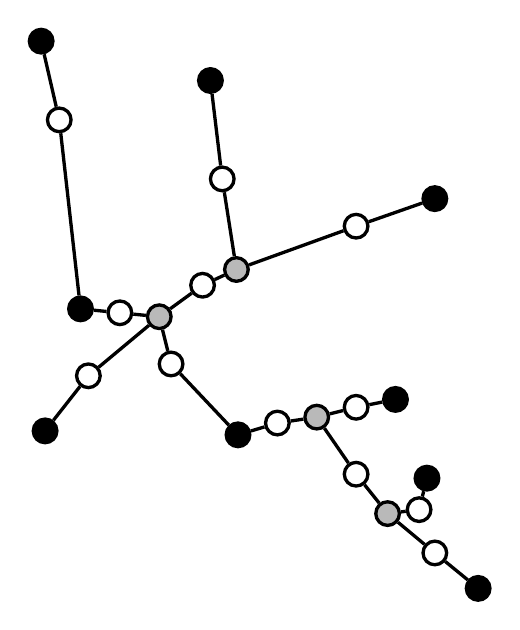
\begin{tikzpicture}[every node/.style={draw, very thick}, every path/.style={very thick}]
    
    \node[circle, draw, minimum size=0.3cm, inner sep=0pt, fill=black] (2) at (-3,4) {};

    
    
    \node[circle, draw, minimum size=0.3cm, inner sep=0pt, fill=black] (4) at (-0.85,3.5) {};
    

    
    \node[circle, draw, minimum size=0.3cm, inner sep=0pt, fill=white] (5) at (-2.77,3) {};
    
    \node[circle, draw, minimum size=0.3cm, inner sep=0pt, fill=white] (6) at (-0.7,2.25) {};
    
    \node[circle, draw, minimum size=0.3cm, inner sep=0pt, fill=black] (8) at (2,2) {};
    
    
    \node[circle, draw, minimum size=0.3cm, inner sep=0pt, fill=white] (10) at (1,1.65) {};
    
    
    \node[circle, draw, minimum size=0.3cm, inner sep=0pt, fill=gray!55] (12) at (-0.52,1.1) {};
    
    \node[circle, draw, minimum size=0.3cm, inner sep=0pt, fill=white] (13) at (-0.95,0.9) {};

    
    \node[circle, draw, minimum size=0.3cm, inner sep=0pt, fill=black] (15) at (-2.5,0.6) {};
    \node[circle, draw, minimum size=0.3cm, inner sep=0pt, fill=white] (16) at (-2,0.55) {};
    \node[circle, draw, minimum size=0.3cm, inner sep=0pt, fill=gray!55] (17) at (-1.5,0.5) {};
    
    \node[circle, draw, minimum size=0.3cm, inner sep=0pt, fill=white] (18) at (-1.35,-0.1) {};

    \node[circle, draw, minimum size=0.3cm, inner sep=0pt, fill=white] (19) at (-2.4,-0.25) {};
    
    
    \node[circle, draw, minimum size=0.3cm, inner sep=0pt, fill=black] (22) at (1.5,-0.55) {};
    
    \node[circle, draw, minimum size=0.3cm, inner sep=0pt, fill=white] (23) at (1,-0.65) {};
    
    \node[circle, draw, minimum size=0.3cm, inner sep=0pt, fill=gray!55] (24) at (0.5,-0.775) {};
    
    \node[circle, draw, minimum size=0.3cm, inner sep=0pt, fill=white] (25) at (0,-0.85) {};

    \node[circle, draw, minimum size=0.3cm, inner sep=0pt, fill=black] (27) at (-2.95,-0.95) {};
    
    \node[circle, draw, minimum size=0.3cm, inner sep=0pt, fill=black] (29) at (-0.5,-1) {};

    
    \node[circle, draw, minimum size=0.3cm, inner sep=0pt, fill=white] (30) at (1,-1.5) {};
    
    \node[circle, draw, minimum size=0.3cm, inner sep=0pt, fill=gray!55] (32) at (1.4,-2) {};
    \node[circle, draw, minimum size=0.3cm, inner sep=0pt, fill=black] (38) at (1.9,-1.55) {};
    \node[circle, draw, minimum size=0.3cm, inner sep=0pt, fill=white] (39) at (1.8,-1.95) {};
    
    \node[circle, draw, minimum size=0.3cm, inner sep=0pt, fill=white] (33) at (2,-2.5) {};
    
    \node[circle, draw, minimum size=0.3cm, inner sep=0pt, fill=black] (35) at (2.55,-2.95) {};
    
    \draw[] (2) to (5);
    \draw[] (4) to (6);
    \draw[] (5) to (15);
    \draw[] (6) to (12);
    \draw[] (8) to (10);
    \draw[] (10) to (12);
    \draw[] (12) to (13);
    \draw[] (13) to (17);
    \draw[] (15) to (16);
    \draw[] (16) to (17);
    \draw[] (17) to (18);
    \draw[] (17) to (19);
    \draw[] (18) to (29);
    \draw[] (19) to (27);
    \draw[] (22) to (23);
    \draw[] (23) to (24);
    \draw[] (24) to (25);
    \draw[] (24) to (30);
    \draw[] (25) to (29);
    \draw[] (30) to (32);
    \draw[] (32) to (33);
    \draw[] (32) to (39);
    \draw[] (33) to (35);
    \draw[] (38) to (39);
    \end{tikzpicture}
    \caption{Auxiliary tree $\mathcal{T}_{\mathcal{Z}}$ built from vertices of set $\mathcal{Z}$. Lines represent edges between vertices of $\mathcal{T}_{\mathcal{Z}}$.}\label{exampleAuxTreeTZ}
\end{minipage}
\end{figure}